\documentclass[11pt]{report}
%%%%%%%%%%%%%%%%%%%%%%%%%%%%%%%%%%%%%%%%%%%%%%%%%%%%%%%%%%%%%%%%%%%%%%
%% uncomment these two lines when running pdflatex (i.e. pdf output)
\usepackage[pdftex]{color}
\usepackage[pdftex,colorlinks,breaklinks,backref]{hyperref}
%%
%% uncomment this line when running normal latex (i.e. dvi output)
%\usepackage{hyperref}
%%
%% comment all three of the above lines for latex2html output
%%%%%%%%%%%%%%%%%%%%%%%%%%%%%%%%%%%%%%%%%%%%%%%%%%%%%%%%%%%%%%%%%%%%%%
%% Using an adapted version of the FEFF doc
%% all the rest of the feffdoc stuff:
\usepackage{feffdoc}
%\usepackage{html} % put after hyperref to avoid conflict in pdf mode

\usepackage{graphicx}
\usepackage{epstopdf}
\usepackage{float}
\usepackage{amsmath,natbib}
\newcommand{\norm}[1]{\left\Vert#1\right\Vert}
\newcommand{\abs}[1]{\left\vert#1\right\vert}
\newcommand{\bra}[1]{\left<#1\right\vert}
\newcommand{\ket}[1]{\left\vert#1\right>}
\newcommand{\braket}[2]{\left<#1\vert#2\right>}
%
\begin{document}

\pagenumbering{roman}
\MakeTitle

\newchapter{}
\begin{abstract}
\program{ocean} is an {\it ab initio} Density Functional Theory (DFT) + Bethe-Salpete Equation (BSE) code for calculations of core-level 
spectra. Currently the code allows for the calculations of x-ray absorption spectra (XAS), x-ray emssion (XES), and non-resonant x-ray 
inelastic x-ray spectra (NRIXS) of periodic systems. The code is written in Fortran 90 with associated shell and Perl scripting.



\vspace*{\stretch{1}}

 \noindent This document is copyright \copyright\ 2010-2015 \program{ocean} collaboration, University of Washington. Following conventions of the FEFF documentation

\end{abstract}

\newchapter{}
\tableofcontents
\newchapter{}

\setcounter{page}{1}
\pagenumbering{arabic}


\chapter{Overview}



\program{ocean} provides a package to numerically solve the Bethe-Salpeter equation for core-level excitations. 
There are several steps in the process which use a variety of compiled programs and scripts. 
The entire processes is driven by the main script \program{ocean.pl}, though the experieced user 
can easily run subsections of the code individually.
The \program{ocean} workflow is as follows:

\begin{enumerate}
\item Setup and parsing of the input file
\item Atomic calculation to construct PAW-style projectors
\item DFT calculation using one of several external DFT codes
\item Calculation to determine the core-hole screening
\item BSE calculation to get the final spectrum or spectra
\end{enumerate}

The guide is broken up into sections to follow the path the code will take. 


\vspace*{\stretch{1}}
\begin{table}[htbp]
  \caption{Typographic conventions in this document}
  \label{tab:typographic}
  \begin{center}
    \begin{tabular}[h]{ll}
      \hline\hline
      \quad font & \quad denotes \\
      \hline
      \program{small caps} & names of programs\\
      \texttt{typewriter font} &  contents of files\\
      \file{quoted typewriter font} & file names\\
      ROMAN CAPITALS & names of cards in the \file{input} file\\
      \texttt{\textsl{slanted typewriter font}} &
      commands executed at a command line \\
      \hline\hline
    \end{tabular}
  \end{center}
\end{table}
\vspace*{\stretch{1}}

\section{Acknowledgments and history}
The \program{ocean} code is based historically off of the NIST BSE codes of Eric Shirley. 
The development of \program{ocean} grew out of  collaboration between Eric Shirley and John Rehr at the University of Washington by way of the thesis project of John Vinson. 

Select \program{ocean} and \program{ocean}-precusor papers (in reverse chronological order) :
\begin{itemize}
\item K.\ Gilmore, \textit{et al.}, (submitted)
\item J.\ Vinson, J.\ J.\ Rehr, J.\ J.\ Kas, and E.\ L.\ Shirley, Phys.\ Rev.\ B \textbf{83}, 115106 (2011)
\item E.\ L.\ Shirley, Ultramicroscopy \textbf{106}, 986 (2006)
\item E.\ L.\ Shirley, Phys.\ Rev.\ Lett.\ \textbf{80}, 794 (1998)
\end{itemize}



The current list of contributors  (in alphabetical order):

\begin{tabular}{l}
Keith Gilmore \\
Josh Kas \\
Das Pemmaraju \\
David Prendergast \\
John Rehr \\
Eric Shirley \\
Fernando Vila \\
John Vinson \\
\end{tabular}

\chapter{Tutorial}

This chapter will run through several tutorials showcasing some of the things \program{ocean} can do and highlighting some of the strategies once can use to make sure a result is ``converged.'' The issue of error estimation in computational physics is a bit beyond this tutorial, but we will focus on what it takes to get a spectrum out of \program{ocean} that is a true representation of the underlying theories and approximations: DFT, pseudopotenials, BSE, \&c. All of the initial inputs can be found in the \file{EXAMPLES} directory. Each section will use a single system to focus on some feature or settings. 

%The purpose of this chapter is to work through a sample \program{ocean} calculation. Go to the \file{EXAMPLES/rutile} directory and look at the file \file{rutile.in}. This is the main input file. For this example let \file{\$OCEAN\_DIR} be the location of the installed \program{ocean} package. Running the command \texttt{\textsl{\$OCEAN\_DIR/ocean.pl rutile.in}} will run ocean. Run this now. If everything runs correctly the main output will be the file \file{CNBSE/absspct} which can be plotted against the included \file{absspct} file to check that the calculation worked.

\section{Quick-start with SrTiO$_3$}

Strontium titanate (STO) is a benchmark perovskite which is widely used experimentally as a substrate, interface, or doped to give interesting properties. 
Computationally it is a good testbed because it is undistorted and both the titanium and strontium are nominally $d_0$. Here we will just be interested in producing a rough calculation of the Ti L$_{2,3}$-edge x-ray absorption of STO.
\begin{itemize}
\item Go to the \file{EXAMPLES/STO} directory
\end{itemize}
All of the necessary files to run should be here. The main input is \file{STO.in} and will require some minor editing before we run. 

When you run \program{ocean} you need to decide how many processors to run on. This can range from 1 on your laptop to thousands on a cluster. {\it Nb.\ When running locally I would recommend selecting fewer processors than your machine has.} You also need to know how your MPI (Message Passing Interface) is called. MPI is what allows the DFT codes to run across many, many nodes on a cluser. Two popular, open-source MPI distributions are \program{mpich} and OpenMPI. To call \program{mpich} you need to use ``mpiexec -n {\it NP''} whereas for OpenMPI the usage is ``mpirun -n {\it NP''} where {\it NP} is the number of processors you want to run on. This information (the wrapper mpiexec/mpirun and {\it NP)} is placed in the input file in \htmlref{PARA\_PREFIX}{card:paraprefix}.

The second choice you will need to make before running is which DFT code you want to use. If only one is installed then your choice is easy. Currently \program{ocean} supports \program{abinit} and \program{QuantumEspresso}. Either should work fine, and for historical reasons the default is \program{abinit}. Selection between the two is accomplished via the \htmlref{DFT}{card:dft}  parameter which can be set to either ``qe'' or ``abi.''
\begin{itemize}
\item Edit \file{STO.in} to reflect your choices for DFT and parallel execution
\end{itemize}
Before looking at any of the other files or settings we want to get the calculation running. 
\begin{itemize}
\item Run \program{ocean}: \texttt{\textsl{/path/to/ocean/ocean.pl STO.in}}
\end{itemize}
While that is running we can look at the other files that were included. First we have the pseudopotential files: \file{*.fhi} and \file{*.fhi.UPF}. Psuedopotentials are covered briefly in chapter \ref{ground_state}. They are necessary for any \program{ocean} calculation. The files \file{ti.opts} and \file{ti.fill} provide a description of the titanium pseudopotential and tell \program{ocean} information about how to construct the matrix elements between the core and the valence electrons (see chapter \ref{paw}). There is also the file \file{photon1} which describes the x-ray experiment being done. In this example we are looking at x-ray absorption, including both dipole and quadrupole terms in the electron-photon interaction. The photon file specifies the direction for the x-ray's polarization $\epsilon$ and momentum $q$ as well as the 
approximant energy (which for the titanium L$_{2,3}$ edge is around 450~eV). A complete description of the photon file format is avaiable in section \ref{photon_files}.

As \program{ocean} runs it will move between several different directories. First it will parse the input file and put all of the settings for the run into the \file{Common} directory. Next it will carry out a series of atomic calculations to determine the localized basis and matrix elements for the core-level to valence excitations in the \file{PAW} directory. The ground-state DFT calculations will be carried out in \file{DFT}, and then a translation into \program{ocean} formatted files will take place in \file{PREP}. The screening of the core-hole potential is done in \file{SCREEN}, and finally the Bethe-Salpeter calculation is carried out in \file{CNBSE}.

\begin{figure}
\center
\includegraphics[angle=270,width=4.5in]{sto_compare.eps}
\caption{ The titanium L$_{2,3}$ edge of strontium titanate as calculated using the STO example. Note the near, but not exact, match between the calculated and supplied spectra. A larger discrepancy might point to a bug or problem with your installation. }
\label{STO_plot}
\end{figure}


When \program{ocean} has finished running there will be files called \file{absspct} in the \file{CNBSE} directory. The naming scheme for these files is straight-forward, but long. Our run will have created the file \file{absspct\_Ti.0001\_2p\_01'}. This means that his \file{absspct} file is for titanium (Ti); it is the first titanium listed in the structure (0001); we ran for the L$_{2,3}$ edge or, equivelantly, the 2$p$ core levels (2p); and the corresponding photon file is \file{photon1} (01). The current \program{ocean} code can support up to 9999 different atomic sites and 99 different photon specifications. {\it If for example you were running on a very large, disordered cell like liquid water and comparing to NRIXS with a dozen different values for the momentum transfer you could run all of them and the outputs would be nicely labeled.}

We need to check the results, so we will plot the resulting \file{absspct\_Ti.0001\_2p\_01} and compare to the included \file{absspct} file in the base \file{STO} directory.
\begin{itemize}
\item Open gnuplot (or your other favorite plotting tool) and compare your spectrum to the included one
\end{itemize}
The two should match very closely, but with the quality settings in the input there may well be differences between the DFT codes (see figure \ref{STO_plot}). The 3{\it d} transition metals highlight the breakdown of a single-particle picture for x-ray absorption. A quick count shows that the intensity ratio between the L$_2$ and the L$_3$ edges should be 2:1 from the intial occupations of the 2$p_{3/2}$ and 2$p_{1/2}$. Instead for titanium we see a ratio of less than 1. The spin-orbit splitting of the 2{\it p} orbitals is not diagonal in the same basis as the conduction band $d$ states, and so trying to move backward from the spectrum to the ground-state density of states (for either the 2$p$ or 3$d$ levels) can be difficult, but the BSE approach in \program{ocean} makes it easy.

\section{Core-level shifts with NH$_4$NO$_3$}

Ammonium nitrate is a wide band gap crystalline solid. Nitrogen atoms occupy central positions in the two constituent ions NH$_4$ and NO$_3$. Given the difference in chemical environment between hydrogen and oxygen nearest neighbors it is of no surprise that there is a significant shift in the energy of the 1{\it s} electrons between the two nitrogen sites. Therefore NH$_4$NO$_3$ makes a good example to look at how we can account for these shifts within \program{ocean}. As always with our tutorials, feel free to start the calculation  and then read while it is running.

There are several methods used for calculating energy levels in core-level spectroscopy. For completeness we will give an overview of them here. The most straightforward, popular in quantum chemistry techniques, is to directly compare the energies of initial and final states. This requires that you calculate explicit initial and final states as well as the core level wavefunction. Pseudopotential-based techniques need a bit more creativity due to their lack of explicit core states. Methods that carry out a self-consistent calculation in the presence of the core hole (full core hole, half core hole, or eXcited core hole) can make use of the energy differences between DFT calculations with and without the core hole. This gives a relative energy shift that can be calibrated to give meaningful information about the core level shifts both within a cell and between different cells.\cite{NeedCites}

The \program{ocean} code has neither explicit core levels or self-consistent calculations with a core hole, and so we need a different approach. In the BSE approach the only elements we need are the bare energies of the electron and the hole, and then the interaction terms. These bare or one-particle energies are the energies that would be calculated within {\it GW}, i.e., the the addition (removal) energies for the conduction electron (core). But a {\it GW} calculation for the core level is neither possible nor feasible, and it is this removal energy we want to try and approximate. Because we are not relaxing the system in the presence of the hole (see the various core-hole approaches mentioned in the previous paragraph) this requires two calculations 1) the energy of the core-level electron and 2) the total energy from the relaxation of the rest of the system once that electron is removed. 

\begin{enumerate}
\item
For calculating the energy of the core level we assume that the core level wavefunction is the same between chemical environments. This means that the kinetic energy of the core level is fixed, and therefore changes in the core-level energy can only come from changes in the local potential. This comes directly from the DFT calculation as the total Kohn-Sham potential.
\item The response of the rest of the system to the removal of the core-level electron is given (within linear response) by the screening of the core-hole potential that we are already calculating. An additional factor of $1/2$ is picked up from adiabatically moving the charge of this electron. 
\end{enumerate}
To evaluate both 1 and 2 we approximate the core as a delta at its location $\tau$. 
The energy of the core hole (as it would then appear in the BSE Hamiltonian $H^0$) is given by
\begin{align}
\epsilon_h = V_\text{KS}(\tau) - 1/2 W(\tau) + X
\end{align}
where X is an offset which will not vary from site to site and encapsulates the core's kinetic energy term and also the sreening response of the other core electrons -- neither of which change from site to site by assumption.

A ground state calculation of ammonium nitrate shows that the bulk of the nitrogen {\it p}-DOS for both the ammonium and nitrate ions is in the same energy region. The nitrate nitrogen has {\it p}-type states that are split into $\sigma$ and $\pi$, and here we are referring to the $\pi$, with the $\sigma$ states significantly lower in energy. In figure \ref{an_xes} we can see the enormous discrepancy between a density of states calculation and the measured x-ray emission. This calculation can be run using the \file{AN} example. What is missing is a calculation of the core-level shifts. 

Core-level shifts are calculated in the screening stage. The parameter XXX controls the calculation. If it is set to ``false'' no calculations are done. If you inspect the \file{AN.in} input file you will see that this is the case for the example. Within \program{ocean} there are three options for this parameter:
\begin{enumerate}
\item false -- don't run any shifts
\item true -- only interested in a single cell
\item $[$ any number $]$ -- will be running many cells, e.g., molecular dynamics snapshots.
\end{enumerate}
Choosing the number to set XXX can be tricky because we have no idea what values the Kohn-Sham potential or screening calculation will give ahead of time. Instead, we can use the option``true" and the code will figure out what value to set XXX to such that the average offset is zero. Go ahead and change the input so that XXX is ``true'' and rerun the calculation. If you'd like you can use the script ``re_run.sh'' by setting the directory where \program{ocean} was installed. 

This time the code has performed additional calculations to get the Kohn-Sham potential at each nitrogen site. The difference is remarkable -- the main parts of the ammonium and nitrate XES are no longer overlapping, but instead separated by several eVs. The core-level shifts are unique to each site and each screening radius. As such they are stored within the \file{SCREEN} directory by site and radius, i.e., \file{SCREEN/zN_01/}. If you look at these files you will see that the two nitrate and two ammonium nitrogens are almost the same (small differences are inevitable) as we expect since they are equivalent sites. 

\iffalse
\section{Rutile}

The main input file, \file{rutile.in}, contains most of the information about the run such as unit cell parameters and numerical parameters. Other important files are the \file{*.fhi} files which contain the pseudo-potentials, the \file{*.fill} and \file{*.opts} files which contain information about the PAW reconstruction, and the \file{jtv1} file which determines information about the probe photon. 

This calculation is definitely not converged, and should not be compared to experiment, any agreement would be fortuitous. Since this is our first time running with either the oxygen or titanium pseudo-potentials we should really check how well the PAW stage performed, but that will be left to a later tutorial. Instead we will start with the screening calculation and work from there. Left out of this tutorial is any investigation of the parameters that determine the quality of the initial DFT runs. For now it is suggested that the user look to ABINIT's provided tutorials to ensure that the calculated DFT wavefunctions are good. The values used in this tutorial are a too stingy for a publication quality run.

\subsection{Screening}

%\begin{figure}
%\includegraphics[scale=0.3]{titanium_screen_radius.pdf}
%\label{titanium_screen_radius}
%\end{figure}


From the rutile working directory drop into the \file{SCREEN/zTi\_01\_n02l01/} directory. This contains the screening information for our run; our atom is titanium (Ti), we are using the first titanium in the cell, and the edge of interest is $n=2;l=1$. In here we see a collection of directories, each corresponding to a different screening calculation. Our first interest is in the behavior of the screening with respect to the cut-off radius for our RPA calculation. Using your favorite plot compare the different \file{ropt} files in the directories \file{zRXT2.00/}, \file{zRXT3.00/}, and \file{zRXT4.00/}. We are interested in comparing columns 1 versus 4, which is the response of the valence electrons to the core-hole potential as a function of radius, all in atomic units. Physically the radius should be taken out to infinity, but we see that the calculation converges relatively quickly. As a note, the radius can not exceed 8 Bohr, and should always be in the vicinity of 2-5~Bohr. Looking at the plot of the three different radii (Fig.\ \ref{rutile_screen_radius}) you will see a large jump between 2 and 3~Bohr but a much smaller jump going to 4. Therefore, by 4~Bohr it appears that the screening calculation is converged, and if you were to compare 3.5 and 4 the difference would be quite small. The parameter CNBSE.RAD sets which screening radius is used by the BSE calculation, and you should set to match the converged radius.


The second thing to check is the number of unoccupied bands used in the screening calculation. Automatically the code will calculate the dielectric function for two different numbers of bands, the number you asked for and a smaller number (some 80\% the size). This smaller calculation is done for each of the radii asked for and is stored in the subdirectory \file{zRXT2.00\_small/}. Having chosen your radius of choice above (4~Bohr) you can check the convergence of the bands by plotting the small and full \file{ropt} files against each other, once again column 1 versus column 4. As you can see in Fig.\ \ref{rutile_screen_bands} there is only a small change going from 75 unoccupied bands down to 60, and so we can consider the calculation to be converged.

%\begin{figure}
%\includegraphics[scale=0.3]{titanium_screen_bands.pdf}
%\label{titanium_screen_bands}
%\end{figure}


\subsection{CNBSE stage}

At this point we will move to the \file{CNBSE} directory and consider the effect of three parameters; NBUSE, CNBSE.XMESH, and NKPT. You might think you missed the parameter NBUSE in \file{rutile.in}, but it is in fact not there. For insulators like rutile it can be determined automatically as the code runs. The BSE section requires that every k-point have the same number of conduction bands in the calculation, but in metals a band can be above or below the Fermi level depending on the k-point. If you look at \file{nbuse.ipt} you will see that it is set to 26. Create a new directory in the run directory called \file{CNBSE\_20/} and edit \file{Common/nbuse.ipt}, changing it to 20. You might notice that it said 0 which tells the code to automatically determine the maximum number of bands available. Here we calculated 50 bands total bands 24 of which are occupied leaving 26. Now go into \file{CNBSE\_20} and run the script \program{cnbse.pl}. This will recalculate the spectra using only 20 bands in the BSE. You can now compare the two spectra files. You'll see that the one with fewer bands falls off at a much lower energy, as is expected. Additionally, it is impossible to tell if 26 bands is enough for convergence, since there are differences between the two spectra. We will have to re-run part of the ABINIT stage, increasing the value of NBAND. Since the convergence with bands should be the same independent of k-point sampling, this step should be done before checking on NKPT.

Another important consideration is the size of CNBSE.XMESH. This determines the number of real-space points in the unit cell that the long-ranged part of the direct interaction is calculated at. Said another way, each DFT wavefunction is truncated down to a small set of Fourier coefficients, and the long-range, spherical direct term is evaluated for each point. This part of the direct term is only a function of the distance between the core hole and the electron position coordinates, $W(|\mathbf{r-r'}|)$. The default should be sufficient for small unit cells, but larger cells will require a bigger mesh. A value of 1-2 points per Bohr of cell length along that direction is typical. 
Changing this parameter, by editing its value in the Common directory requires re-running the PREP stage as well as the CNBSE stage. 
%If you edit it in the input file and re-run the whole calculation it might work, but there may also be bugs either causing too much or too little to be re-run. 
Indeed, if you check, you will see that a $4\times4\times4$ grid is insufficient, and there are large deviations if you increase to a $6\times6\times6$ grid. But increasing it further will change little, showing that 216 x-points are sufficient. 

%\begin{figure}
%\includegraphics[scale=0.5]{titanium_xmesh.pdf} \\
%The convergence of the spectra with respect to the number of x-points, ie. cnbse.xmesh.
%\label{titanium_xmesh}
%\end{figure}

The parameter NKPT determines the number of k-points used in the BSE. \program{ocean} uses, by default, a very asymmetric shift to ensure that the k-points sampled are fairly unique. The number of k-points varies widely from system to system, with metals or small unit cells using 4096 or more points, while large systems might need only 8-64. The mesh does not need to use the same number for each element, and for oblong unit cells should not, but all the meshes in \program{ocean} should be factorable into small primes; 2, 3, or 5. The default tutorial mesh was $4\times4\times2$ which is too small, but faster to run [ALSO THIS SHOULD BE 224]. Try increasing the number of k-points, but try and match your grid to the ratio of reciprocal lattice vectors, about 1.5:1. 

This concludes the tutorial on rutile TiO$_2$.

\fi




\chapter{Inputs}

The \program{ocean} package is run using the \program{perl} script \program{ocean.pl} which takes care of reading in the input file and then running the various executables. This chapter will introduce the various controls and explain their formatting and use.


\section{Running \OCEAN}

In addition to the main input file there are several auxiliary files. The \file{*.opts} and \file{*.fill} files are described in sections \ref{opts}  and \ref{fill} respectively, and the pseudopotentials are touched upon briefly in chapter \ref{ground_state}. The next section, \ref{photon_files}, covers the \file{photon?} files which specify the necessary information about the x-ray probe. 

The input parser for \program{ocean} is relatively basic. Any text following a comment character, `\#,' is ignored up to the line return. If a file has been switching around operating systems it may have non-unix line returns which can cause problems. If the parser returns odd errors try running \program{dos2unix}. The parser is case ignoring and converts all inputs to lower case, requiring any filenames in the input file to be lower case. Each card must be on its own line followed by the value or values to be assigned it. All card values can be surrounded by braces (\{\}) and multi-value cards must be surrounded by braces. For example, the NKPT card must be a list of 3 integers and so must have the following form: ``NKPT \{ 2 2 2 \}" whereas the OCCOPT card takes only one integer and may therefore be listed: ``OCCOPT 1" or ``OCCOPT \{ 1 \}". Line returns may be present within an input. 

After parsing the cards are all stored as small, fortran formatted files in the \file{Common} directory. The package then goes through the following steps:
\begin{enumerate}
\item An atomic calculation is done to create projectors following the PAW method.
\item Slater F and G integrals are computed at the atomic level
\item \program{abinit} or \program{QuantumEspresso} input files are prepared
\item \program{abinit} (or \program{QuantumEspresso}) is run to get DFT valence density and wavefunctions. This requires usually 3 runs. One self-consistent run to get the converged density and two additional runs to calculate wavefunctions for the screening calculation and for the final states.
\item The wavefunctions and density are converted from \program{abinit} (or \program{qe})  output to the form expected by \program{ocean}.
\item The core electrons are screened self-consistently in the presence of the core-hole in the atomic system
\item The spherical part of the direct interaction is screened using RPA. $\chi^0$ is calculated using real-space integration around the site of interest. The RPA is coupled with a form of the Levine-Louie-Hybersten screening model.
\item The overlap is calculated between the core wavefunction and the conduction band using the specified photon operator, XAS or RXIS.
\item The Bethe-Salpeter equation (BSE) is iteratively solved using a form of the Haydock recursion algorithm.
\end{enumerate}

\section{Photon files}
\label{photon_files}
The \file{photon} files determine the specifics of the x-ray operator. A single \program{ocean} 
calculation may involve a single \file{photon} file or many, depending on the experiment in question. 
There is currently a hard limit of 99 (which may be excessive), and each should be numbered. 

As an example, if one is simulating non-resonant inelastic x-ray scattering NRIXS (also called x-ray Raman or XRS) 
the experiment being compared to may include a dozen different values for the momentum transfer. 
This is easily done with \program{ocean} and the user needs simply to create 12 files 
named \file{photon1} through \file{photon12}.  

\subsection{Photon operators}
In \program{ocean} we currently support 3 photon operators: 
\begin{itemize}
\item dipole: $\hat{\epsilon} \cdot \mathbf{r}$
\item quad: $\hat{\epsilon} \cdot \mathbf{r} + i/2 \left( \hat{\epsilon} \cdot \mathbf{r} \right) \left(\mathbf{q} \cdot \mathbf{r} \right)$
\item NRIXS: $e^{i \mathbf{q} \cdot \mathbf{r} }$
\end{itemize}
For most light elements the combination of a small core 
wave-function (small $\mathbf{r}$) and small photon energy (therefore small $\mathbf{q}$) 
conspire to make dipole and quad effectively the same, i.e., they are in the dipole limit. 
If you are ever unsure just make two \file{photon} files and check!

\subsection{Photon format}
Below is a sample \file{photon} file. Note that for the photon file, 
depending on the calculation, only some of the information in it will affect the calculation. 
Look back to the operators in the previous section. They don't use all the same variables. 

\begin{center}
\begin{tabular}{| l | c c|}
\hline
dipole				& & operator \\
\hline
cartesian  0  0  1		& & $\hat{\epsilon}$  \\
end			& & \\
\hline
cartesian  0  1  0		& & $\hat{q}$  \\
length 8.55 inverseangstroms && $\vert \mathbf{q} \vert$ \\
end			& & \\
\hline
9000 & & X-ray energy (eV) \\
\hline
\end{tabular}
\end{center}

The file has four sections. In the first we select our operator. 
In the second we set the direction for the x-ray polarization vector $\epsilon$ (currently no circularly polarized light). 
The next section's meaning depends on the operator in play. 
For quad it sets the $q$-vector direction for the incoming light, 
while for NRIXS it sets the direction and magnitude of the momentum \textbf{transfer} 
(the length specifier is optional unless NRIXS is selected). For dipole the $q$-vector doesn't enter in. 
The fourth section is only important for quad and it sets the magnitude of $q$ by way of the photon's energy in eV. 

\section{Complete list of \program{ocean} inputs}

The input of \program{ocean} can be divided into several sections

\begin{itemize}
\item run info
\item structural information of the material
\item non-structural DFT parameters, e.g., convergence
\item atomic and screening info
\item parameters that control the BSE section and its convergence
\item parameters that only affect the output spectrum
\end{itemize}


\begin{description}

  %%
  %% STRUCTURAL INFORMATION
  \item[\large\textbf{Run Control}]\dotfill\
  \begin{description}
    \item[\textbf{Purpose:}] Control aspects of the run
 \item[\textbf{Optional Cards:}] 
    \htmlref{PARA\_PREFIX}{card:paraprefix}, \htmlref{DFT}{card:dft}, 
    and \htmlref{SCRATCH}{card:scratch}
\end{description}
\item[\large\textbf{Structural information}]\dotfill\
  \begin{description}
  \item[\textbf{Purpose:}] Specify the structure
  \item[\textbf{Required Cards:}] 
    \htmlref{ACELL}{card:acell},
    \htmlref{RPRIM}{card:rprim},
    \htmlref{NTYPAT}{card:ntypat},
    \htmlref{ZNUCL}{card:znucl},
    \htmlref{NATOM}{card:natom},
    \htmlref{TYPAT}{card:typat},
    \htmlref{XRED}{card:xred},
    and \htmlref{DIEMAC}{card:diemac}
  \end{description}
\item[\large\textbf{Non-Structural DFT parameters}]\dotfill\
  \begin{description}
  \item[\textbf{Purpose:}] Control convergence of the DFT calculation
  \item[\textbf{Required Cards:}] 
    \htmlref{PP\_LIST}{card:pp_list} and
    \htmlref{ECUT}{card:ecut}
  \item[\textbf{Recommended Cards:}] 
      \htmlref{NKPT}{card:nkpt},
    \htmlref{NGKPT}{card:ngkpt},
        \htmlref{NBAND}{card:nband},
     \htmlref{PAW.NBAND}{card:paw.nband},
    \htmlref{OCCOPT}{card:occopt}, \\
    and \htmlref{FBAND}{card:fband}
  \item[\textbf{Optional Cards:}] 
    \htmlref{TOLDFE}{card:toldfe},
    \htmlref{TOLWFR}{card:tolwfr}, 
    \htmlref{PAW.NKPT}{card:paw.nkpt},
    \htmlref{ABPAD}{card:abpad}, 
    \htmlref{BSE\_ENERGY\_RANGE}{card:bse_energy_range},
    and \htmlref{PAW\_ENERG\_RANGE}{card:paw_energy_range}
  \end{description}
\item[\large\textbf{Atomic and Screening Info}]\dotfill\
  \begin{description}
  \item[\textbf{Purpose:}] Controls the PAW and screening sections of the calculation
  \item[\textbf{Required Cards:}] 
    \htmlref{PAW.FILL}{card:paw.fill},
    \htmlref{PAW.OPTS}{card:paw.opts},
    \htmlref{NEDGES}{card:nedges},
    and \htmlref{EDGES}{card:edges}
  \item[\textbf{Recommended Cards:}] 
     \htmlref{PAW.SHELLS}{card:paw.shells},
     \htmlref{CNBSE.RAD}{card:cnbse.rad}, and 
     \htmlref{SCFAC}{card:scfac}
  \item[\textbf{Optional Cards:}]     
     \htmlref{PAW.HFKGRID}{card:paw.hfkgrid}
  \end{description}
\item[\large\textbf{BSE Parameters}]\dotfill\
  \begin{description}
  \item[\textbf{Purpose:}] Parameters used in the BSE calculation
  \item[\textbf{Recommended Cards:}]   
    \htmlref{CNBSE.XMESH}{card:cnbse.xmesh} and \htmlref{CNBSE.MODE}{card:cnbse.mode}
  \item[\textbf{Optional Cards:}]   
    \htmlref{METAL}{card:metal},
    \htmlref{CKS.STRETCH}{card:stretch},
%    \htmlref{CKS.NORMAL}{card:cks.normal},
    and  \htmlref{CNBSE.STRENGTH}{card:strength}
  \end{description}
\item[\large\textbf{Spectrum Information}]\dotfill\
  \begin{description}
  \item[\textbf{Purpose:}] Controls the spectrum that is written out, not any aspect of the actual calculation
  \item[\textbf{Recommended Cards:}]   
    \htmlref{CNBSE.BROADEN}{card:broaden}  
   \item[\textbf{Optional Cards:}]   
    \htmlref{CNBSE.SPECT\_RANGE}{card:spect-range},
    and \htmlref{CNBSE.NITER}{card:niter}
  \end{description}   
\end{description}

These CARDS are listed below in (almost) the same order as in the table above.
Each CARD description is of this form:

\begin{Card}{CARD}{required arguments}{type}{}
\end{Card}
or \\
\begin{Card}{CARD}{required argument list[ length of list ]}{type}{}
  The type is one of \textsl{Required}, \textsl{Recommended}, or
  \textsl{Optional}. The argument list is a brief statement of the
  valid arguments to the card. Arguments in square brackets are 
  optional. The text description explains the arguments and 
  their uses more fully. Example uses of the card look like this:
\begin{verbatim}
  * brief description of the example
  CARD  arguments
\end{verbatim}

For arguments that are 2-D arrays the ordering is in normal math / C ordering.
\end{Card}

\section{Run Control}
\label{sec:Run-Control}

\begin{Card}{PARA\_PREFIX}{para\_prefix}{Optional}{paraprefix}
This is necessary for parallel runs. Depending on your system you may need so helper to launch parallel jobs such as \program{mpirun}, 
\program{mpiexec}, or \program{aprun}. The \program{ocean} scripts are designed to try and parse this to figure out how many processors 
you are trying to run across, e.g., `mpirun -n 12' will be parsed to tell \program{ocean} to prepare DFT runs across 12 cores. 
\end{Card}

\begin{Card}{DFT}{dft}{Optional}{dft}
This controls which DFT code to use by specifying either `qe' for \program{QuantumEspresso} or `abi' for \program{abinit}. 
By default \program{abinit} is used.
\end{Card}

\begin{Card}{SCRATCH}{scratch}{Optional}{scratch}
Recommended for compute clusters with local scratch space so that \program{abinit} or \program{Quantum Espresso} 
will write scratch files somewhere reasonable. The path \file{scratch} should include an absolute path. Otherwise the default 
behavior is that scratch files will be written to the \file{DFT} directory. 
\end{Card}


\section{Structural Information}
\label{sec:Structural-Information}



\begin{Card}{ACELL}{acell[ 3 ]}{Required}{acell}
  ACELL sets the scaling (in Bohr) for the primitive vectors of the unit cell which are in turn set by \htmlref{RPRIM}{card:rprim}.

\begin{verbatim}
  * For Li metal: BCC structure, a = b = c = 6.595 Bohrs
  ACELL { 6.595  6.595  6.595 }
  
  \end{verbatim}
\end{Card}

\begin{Card}{RPRIM}{rprim[ 3 ][ 3 ] }{Required}{rprim}
  RPRIM sets the primitive vectors for defining the unit cell. 
  
  \begin{verbatim}
  * For a BCC
  RPRIM{ 1.0  0.0  0.0
         0.0  1.0  0.0
         0.5  0.5  0.5  }
  
  * or the more symmetric
  RPRIM{ -0.5  0.5  0.5
          0.5 -0.5  0.5
          0.5  0.5 -0.5  }
         
  \end{verbatim}
\end{Card}

\begin{Card}{NTYPAT}{ntypat}{Required}{ntypat}
The card NTYPAT gives the number of different types of atoms in the cell. 
\end{Card}

\begin{Card}{ZNUCL}{znucl[ntypat]}{Required}{znucl}
\texttt{znucl}[] is a list of length \texttt{ntypat} that gives the atomic numbers of the types of atoms that are in the cell.
\end{Card}

\begin{Card}{NATOM}{natom}{Required}{natom}
The card NATOM gives the number of total atoms in the cell.
\end{Card}

\begin{Card}{TYPAT}{typat[natom]}{Required}{typat}
The card TYPAT lists each atom by the rank it has in the \htmlref{ZNUCL}{card:znucl} list. The order they are listed in will correspond to \htmlref{XRED}{card:xred}. (This may be fixed soon to be less idiosyncratic.)
\end{Card}

\begin{Card}{XRED}{xred[natom,3]}{Required}{xred}
The XRED card lists the reduced coordinates, ( x, y, z ), of the all \texttt{natom} atoms in the cell.
  \begin{verbatim}
  * For a diamond-like structure with 2 atoms per unit cell
  XRED{ 0.0  0.0  0.0    # atom 1
        0.25 0.25 0.25 } # atom 2
  \end{verbatim}
\end{Card}

\begin{Card}{DIEMAC}{diemac}{Required}{diemac}
The MACropscopic DIElectric constant \texttt{diemac} is required for both the DFT stage and also as a parameter in the screening calculations. It is included here as a physical property of the system of interest.
\end{Card}

%%%%%%
\section{DFT Parameters}
\label{sec:DFT-Parameters}

%%% DFT: Required

\begin{Card}{PP\_LIST}{files[ntypat]}{Required}{pp_list}
The names of the pseudo-potential files need to be listed here in the same order as \htmlref{znucl}. Currently all these files need to be all lower case.
\end{Card}

\begin{Card}{ECUT}{ecut}{Required}{ecut}
The plane-wave basis is truncated according to \texttt{ecut} measured in Rydberg. The plane-wave cut-off is determined mostly from the pseudo-potentials being used and convergence should be checked with respect to ground state energy.
\end{Card}

%%%% DFT:Reccomended
\begin{Card}{NKPT}{nkpt[3]}{Recommended}{nkpt}
NKPT sets the number of k-points used to sample the cell for calculation of the final states. The required number of k-points will vary based on system size (inversely with unit cell volume), and in general metals will require larger grids than insulators. Convergence should always be checked against the k-point sampling. If this is not specified than \program{ocean} will attempt to guess at a reasonable value. 
\end{Card}

\begin{Card}{NGKPT}{ngkpt[3]}{Recommended}{ngkpt}
DFT calculations require a self-consistently determined ground state density for the Kohn-Sham Hamiltonian. As such, in \program{ocean}, first a ground state calculation is done using only the occupied states and a few unoccupied states for convergence. This density is then used as input to the other DFT calculations to get wavefunctions. NGKPT determines the k-point sampling for this ground state calculation. Care should be taken to ensure enough k-points are used to give a converged density.
\end{Card}

\begin{Card}{NBAND}{nband}{Recommended}{nband}
The number of total bands for the final-state wave-functions is set by NBAND. This includes all valence states but not core states.
\begin{verbatim}
  * In diamond there are two C atoms each with 4 valence electrons.
  * To include only the bottom 4 conduction bands
  nband 8
\end{verbatim}
\end{Card}

\begin{Card}{PAW.NBAND}{paw.nband}{Recommended}{paw.nband}
PAW.NBAND sets the number of bands to be calculated for the screening wave-functions. The screening calculation requires a large number of bands as the screened potential only converges in the \texttt{paw.nbands} $\rightarrow \infty$ limit. In practice including bands around 100~eV above the fermi level should be sufficient, but convergence should be checked. 
\end{Card}

\begin{Card}{OCCOPT}{occopt}{Recommended}{occopt}
OCCOPT controls how \program{ABINIT} determines occupation. The allowed values of \texttt{occopt} are listed in the \program{ABINIT} documentation, but the two most important are 1 and 3 as spin-dependent DFT is not yet compatible with \program{ocean}.
\begin{description}
\item[\texttt{occopt} = 1]\hfill\\ States are all doubly degenerate and either occupied or empty depending on band. Suitable for insulators. 
	For \program{Quantum Espresso} this is equivalent to  OCCUPATIONS = `fixed'.
\item[\texttt{occopt} = 3]\hfill\\ States are all doubly degenerate but can have fractional occupations depending on fermi level. Suitable for metals. For \program{Quantum Espresso} this is equivalent to OCCUPATIONS = `smearing'. 
\end{description}
\end{Card}

\begin{Card}{FBAND}{fband}{Recommended}{fband}
FBAND determines the number of unoccupied bands to be included in the SCF calculation of the density. For insulators the default (\texttt{fband} = 0.125) is fine, but for metals care must be made to ensure that the highest band in the density calculation has no occupation weight. The number of extra bands is determined by the formula n = \texttt{natom} * \texttt{fband}. Current this is only enabled for the \program{ABINIT} version of the code. The \program{Quantum Espresso} version will only use the defaults. 
\end{Card}

%%% DFT: Optional

\begin{Card}{TOLDFE}{toldfe}{Optional}{toldfe}
TOLDFE sets the convergence parameter for the density or SCF run. For \program{abinit} when the total energy changes by less than \texttt{toldfe} in two consecutive SCF runs the density is assumed to be converged. The default (\texttt{toldfe} = $10^{-6}$) might be a little too permissive, but is adequate for many systems. For \program{Quantum Espresso} this sets the CONV\_THR parameter for the SCF calculation. 
\end{Card}

\begin{Card}{TOLWFR}{tolwfr}{Optional}{tolwfr}
The convergence criterium for the (NSCF) wave-function calculations is set by TOLWFR. The default (\texttt{tolwfr} = $10^{-16}$) should be sufficient. For the \program{Quantum Espresso} version, this parameter sets the CONV\_THR for the NSCF calculations. 
\end{Card}

\begin{Card}{PAW.NKPT}{paw.nkpt[3]}{Optional}{paw.nkpt}
The screening calculation is less sensitive to k-point sampling than the final states and is therefore calculated on a smaller grid which is set by PAW.NKPT. The default setting ( PAW.NKPT = 2 2 2 ) is sufficient for a wide variety of systems though very small or very large unit cells may require more or only the gamma point respectively. 
\end{Card}

\begin{Card}{ABPAD}{abpad}{Optional}{abpad}
During the non-self-consistent calculation of the wavefunctions, the convergence of the highest bands can be very slow. The calculation speed can be increased by adding some throw-away bands to the top. These bands are not considered when checking for convergence and should also not be used in the subsequent steps of the calculation. The parameter abpad adds bands to the calculation and tells ABINIT to ignore them using ABINIT's nbdbuf setting. This has no effect for the \program{Quantum Espresso} version. 
\end{Card}

\begin{Card}{BSE\_ENERGY\_RANGE}{bse\_energy\_range}{Optional}{bse_energy_range}
Instead of setting the number of bands (\texttt{nband}) the user may request an energy range in eV for the final-state wave-functions. 
This is only an estimate using the volume of the unit cell and may be unreliable. 
This parameter is only used if no value for \texttt{nband} is given. The default value is 25~eV.
\end{Card}

\begin{Card}{PAW\_ENERGY\_RANGE}{paw\_energy\_range}{Optional}{paw_energy_range}
Instead of setting the number of bands for the screening (\texttt{paw.nband}) the user may request an energy range in eV. 
This is only an estimate using the volume of the unit cell and may be unreliable. 
This parameter is only used if no value for \texttt{paw.nband} is given. The default value is 100~eV. 
\end{Card}

%%%%%%
\section{Atomic and Screening Info}
\label{sec:AS-Info}

\begin{Card}{PAW.FILL}{z z.fill}{Required}{paw.fill}
Each type of atom you want spectra of requires a \file{*.fill} file which is explained in \ref{fill}. Eventually the code will handle doing an arbitrary set of edges for a given system so this input could have as many (\texttt{z} \texttt{z.fill}) pairs as you have types of atoms, \texttt{ntypat}. Right now you MUST only put one type here due to bugs. The file \file{z.fill} can in principle have any name, but it is recommended a reasonable naming scheme is kept that associates it with a specific pseudo-potential file. The number \texttt{z} is the atomic number of the site of interest.

\begin{verbatim}
  * Looking at Oxygen K-edge
  8  o.fill
\end{verbatim}
\end{Card}

\begin{Card}{PAW.OPTS}{z z.opts}{Required}{paw.opts}
Each type of atom you want spectra of requires a \file{*.opts} file which is explained in \ref{fill}. Eventually the code will handle doing an arbitrary set of edges for a given system so this input could have as many (\texttt{z} \texttt{z.opts}) pairs as you have types of atoms, \texttt{ntypat}. Right now you MUST only put one type here due to bugs. The file \file{z.opts} can in principle have any name, but it is recommended a reasonable naming scheme is kept that associates it with a specific pseudo-potential file. The number \texttt{z} is the atomic number of the site of interest.

\begin{verbatim}
  * Looking at Oxygen K-edge
  8  o.opts
\end{verbatim}
\end{Card}

\begin{Card}{NEDGES}{nedges}{Required}{nedges}
The number of edges to run is set by NEDGES. Each site and edge is counted separately. So for a 64 atom amorphous carbon cell you would want \texttt{nedges} = 64 for a complete sample. To run the K and L edges Titanium edges in TiS$_2$ you would need \texttt{nedges} = 3. See also \htmlref{EDGES}{card:edges}.
\end{Card}

\begin{Card}{EDGES}{edges[nedges,3]}{Required}{edges}
Each edges being run is defined by 3 integers that set which atom in the same order as \htmlref{XRED}{card:xred}, and which initial state by $n$ and $l$. Note, spin-orbit split edges are calculated together as is necessary to include multiplet terms.

For example, running TiS$_2$ where Ti was listed as the first atom and looking at the K, L$_1$, and L$_{2,3}$ edges respectively.
\begin{verbatim}
  * atom, n, l
    Ti    1  0
    Ti    2  0
    Ti    2  1
\end{verbatim}
\end{Card}

\begin{Card}{PAW.SHELLS}{shells[]}{Recommended}{paw.shells}
The screening calculation is a hybrid of RPA and a model based off of Levine-Louie-Hybersten see section \ref{screening}. The corss-over between these two regimes is set by \texttt{shells} in Bohr and several different radii can be chosen to look at the convergence. In the \texttt{shells} $\rightarrow \infty$ limit the RPA is being used for the entire calculation, but convergence is usually reached around 3 - 4 Bohr. If a large radius is being used than the supercell defined by \htmlref{PAW.NKPT}{card:paw.nkpt} must have dimensions larger than the radius chosen or the math could be odd. The default \texttt{shells} = 1.5 Bohr is not recommended.

This parameter should not exceed 6~Bohr in the current version of the code.
\end{Card}

\begin{Card}{CNBSE.RAD}{cnbse.rad}{Recommended}{cnbse.rad}
One screening radius as defined by \htmlref{PAW.SHELLS}{card:paw.shells} is used in the BSE calculation and is specified by CNBSE.RAD. 
\end{Card}

\begin{Card}{SCFAC}{scfac}{Recommended}{scfac}
The Slater integrals are calculated in an atomic program and are generally scaled by some factor before use. For 3d transition metals a value of $0.8$ is often used, while for $f$-electron atoms a value of $0.6$ may be more appropriate. The value is more or less taken to be independent of the chemical environment and only a function of the element in question.
\end{Card}

\begin{Card}{PAW.HFKGRID}{paw.hfkgrid}{Optional}{paw.hfkgrid}
This sets two parameters for the program \program{hfk.x}. The first is a grid and should be left at the default value of 2000. The second determines the maximum number of projectors per angular momentum channel that can be created. In the future this should dynamically resize, but in the present the default of 20 will work for many calculations. If the program \program{hfk.x} fails it may be solved by increasing this number. It will say something about `ne' being too small. 
\end{Card}


%%%%%%
\section{BSE Parameters}
\label{sec:BSE-Parameters}

\begin{Card}{CNBSE.XMESH}{xmesh[3]}{Recommended}{cnbse.xmesh}
When the wave-functions are converted into the NIST BSE format they are condensed onto a grid controlled by CNBSE.XMESH. The states are then projected onto a localized basis set, using the PAW formalism. By default \program{ocean} will attempt to guess a reasonable 
setting for this mesh. 
%The default(\texttt{xmesh} = 6 6 6) might be insufficient for large unit cells.
\end{Card}

\begin{Card}{CNBSE.MODE}{mode}{Recommended}{cnbse.mode}
The mode can be either ``XAS'' or ``XES'' (NRIXS or XRS are treated the same as XAS). By default the code uses ``XAS.''
\end{Card}

\begin{Card}{METAL}{metal}{Optional}{metal}
The METAL card determines wether the code expects to determine occupation by band or by energy with respect to the fermi energy. The parameter \texttt{metal} can be set to either $.true.$ or $.false.$ (default). If \texttt{metal} is set to {\it .true.} the code will complain unless \htmlref{OCCOPT}{card:occopt} is 3 and similarly for \texttt{metal} = {\it .false.} and \texttt{occopt} = 1. The use of \program{ocean} on metals requires some further testing. 
\end{Card}

\begin{Card}{CKS.STRETCH}{cks.stretch}{Optional}{stretch}
An approximation to some kind of self-energy is allowed through the use of CKS.STRETCH. All conduction band energies with respect to the fermi level are multiplied by \texttt{stretch}. By default \texttt{stretch} = $1.0$. 
\end{Card}

\begin{Card}{CNBSE.STRENGTH}{cnbse.strength}{Optional}{strength}
This card sets the strength for the two interaction terms in the BSE Hamiltonian. By default it should be set to $1$, and for emission the code automatically sets it to $0$. 
It can be changed for curiosity's sake.
\end{Card}

%\begin{Card}{CKS.NORMAL}{cks.normal}{Optional}{cks.normal}
%This determines wether we are considering absorption or emission. The default value of {\it .true.} is appropriate for XAS or NRIXS
%while XES is specified by choosing {\it .false.}.
%\end{Card}


%%%%%%
\section{Spectrum Information}
\label{sec:Spectrum-Information}
\begin{Card}{CNBSE.BROADEN}{broadening}{Recommended}{broaden}
The amount of Lorentzian broadening included in the spectra is set by CNBSE.BROADEN. This is a required convergence parameter for the continued fraction that is our Haydock approximation to the BSE, but setting it to the core-hole intrinsic broadening is recommended since features sharper than that won't be observable. Given in Hartree the default is \texttt{broadening} = $0.007$~Ha. or about $0.1$~eV.
\end{Card}

\begin{Card}{CNBSE.SPECT\_RANGE}{esteps emin emax}{Optional}{spect-range}
This controls the output spectrum (or spectra) from a run. The energy of the specturm is set by setting the conduction band minimum and core-hole binding energy to zero. All systems will include a small amount of excitonic binding (depending on $l$ selection rules) and spin-orbit splitting can lower the first peak significantly, eg. L$_{2,3}$ splitting in 4d transition metals. These parameters do not change the BSE calculation, only the output of the spectra at the end. The energy range is given in eV and by default \texttt{emin} = $-40.817$ and \texttt{emax} = $68.028$ ($-1.5$ to $2.5$ Ha.). The parameter \texttt{esteps} gives the number of energt points used for the plot, and by default it is $1200$.
\end{Card}

\begin{Card}{CNBSE.NITER}{niter}{Optional}{niter}
This sets the number of Haydock iterations. The default is $100$.
\end{Card}





%%%%%%%%%%%%%%%%%%

%\chapter{Additional Input Files}
%In addition to the main \program{ocean} input file there are several files required for a calculation. These are the *.opts, *.fill, photon, and pseudopotentials. This chapter will cover the first three, and psuedopotentials will be covered briefly in the next chapter.
%
%\section{*.opts and *.fill Files}
%The fill and opts files 

\chapter{Ground-State Wavefunctions}
\label{ground_state}
In principle any pseudo-potential DFT code can be used. In our implementation we have an interfaces for using 
\program{abinit} \cite{abinit0,abinit1,abinit2,abinit3} and \program{QuantumEspresso} \cite{espresso1,espresso2}. 
%To run with a custom format see the specs listed in Appendix~\ref{WF_format}.

There are two important differences between what is required for a good core-level calculation with \program{ocean} and more traditional ground-state DFT calculations. The first is that spectroscopy calculations often require denser $k$-point sampling than a calculation of only the density. Secondly, a psuedo-potential that is suitable for ground-state calculations may have poor scattering characteristics at higher energies that will make up the spectrum being calculated. With these brief warnings the rest of this chapter will be spent going over various aspects of the calculation and mention briefly strategies for ensuring accuracy and convergence.

%The user is assumed to be familiar with DFT calculations, ie. converging the total energy or unit cell volume. 
You need a structure and a set of pseudo-potentials to begin a calculation. From there, you must check convergence with respect to all of the adjustable parameters of the calculation. Not to worry, there are not really that many. In this section we will focus on just a few.

\section{Pseudo-potentials}

Pseudo-potentials must be carefully constructed to ensure that they adequately mimic the all-electron system being investigated. For general purpose pseudo-potentials this means having good transferability so they can be used in a variety of chemical environments. Some literature exists on the topic, and the reader is invited to read up on it\cite{Psp} .

As mentioned above for excited state calculations states as high as 50-100~eV above the fermi level must be adequately represented by the pseudo-potentials used. This often requires a harder pseudo-potential than might otherwise be necessary for 
other calculations. Additionally the way in which chemical bonding affects the valence and low-lying conduction bands is often influenced by the inclusion of semi-core states in the calculation. Better agreement is often seen with the inclusion of semi-core states, eg. 2s and 2p states in a 3d transition metal. This has been seen to also improve the high-energy scattering.\cite{}

In the future the authors hope to collect a database of pseduo-potentials to add to the ease of using \program{ocean},
 and all users will be invited to contribute their carefully tested ones as well. Currently the format of the pseudopotentials must
 match that of  .fhi. Users can download compatible pseudopotentials from the \program{abinit} website \cite{abinit0} or build their own using the \program{opium} code. 

\section{Self-consistent Density Calculation}
A DFT calculation requires, as one might expect, a density. In the self-consistent loop, wavefunctions are converged in an inner loop, and the density is updated from there to form an outer loop. Once the density has been converged, in this usage it changes less than the parameter TOLDFE over the course of two successive updates, this calculation is complete. The density, $n(\mathbf{r})$, depends on two (2) major convergence factors; ECUT and NGKPT. What follows is a brief discussion of these and other parts of the density calculation.

In plane-wave based codes the basis size is truncated according to the ECUT parameter, specifying the largest energy plane-wave. This cut-off energy is largely dominated by the pseudo-potentials, the harder the pseudo-potential the higher the cut-off energy needs to be. It should be noted that the scaling of the DFT section with respect to the number of planewaves is no better than N*LOG(N), and the number of planewaves goes as the cut-off to the 3/2 power. When the total energy no longer changes as a function of an increasing energy cut-off the calculation is converged. A reasonable value would be 1meV per atom or less.

The second important factor is the k-space sampling used for the self-consistent calculation. As in all numerical work, integrations are replaced by finite sums. The required k-space sampling is highly material dependent. A material with a small unit cell or a metal will both tend to require a larger number of k-points. This can be guided by experience, but should always be checked by increasing the sampling and looking at the total energy or perhaps the pressure. 

The last consideration is the treatment of electron occupancies. For insulators this is straightforward, fill all the lowest bands, but for metal the situation requires more care. Choosing a value of OCCOPT that is greater than 1 will cause \program{abinit} to smear the occupation levels near the fermi energy. This helps lead to faster convergence by better sampling the fermi surface. Along with metallic occupations comes the need to include enough extra bands in the density calculation to hold the smeared out electrons. The parameter FBAND determines how many extra bands are added. These two parameters follow directly from their \program{abinit} definitions and more can be found in \program{abinit}'s help. When using \program{QuantumEspresso} smearing is always enabled, but this may change in the future. 




\section{K-point sampling}

A sum over a few wavefunctions $\psi_k$ is substituted for a integral over the entire Brillouin zone. In principle knowledge of the crystal symmetry of the unit cell could allow for intelligent choices of  points to sample at with non-equal weight, but that is not the approach here. Instead a regular mesh of points in reciprocal space is used and the mesh must be dense enough to ensure that the sampling is sufficient. 

In practice the required $k$-point grid scales inversely with unit cell size, but testing runs at different sizes and checking that the spectrum is unchanged should be done for each calculation. Unit cells that are oblong may benefit from k-point meshes that have a larger number of k-points along the dimensions with longer {\bf reciprocal} lattice vectors. The only way to ensure convergence w.r.t.\ $k$-point sampling is to increase or decrease the number of $k$-points and make sure that the results are not changing. For metals a large number of k-points may be required in order to get a good sampling of the Fermi surface.

\section{Number of Bands}

The excited state (excitonic) wave-function at any given energy may include contributions from much higher energy DFT wave-functions. Additionally the attractive core-hole potential will pull some states down in energy. If one is interested in spectra up to 20~eV above the edge, the number of bands needed in the calculation will be larger than if one is only interested in the DOS up to 20~eV. This convergence should be tested explicitly. 
%Ref tutorial section once it exists

\section{Beyond DFT}

In principle these wave-functions should include self-consistent self-energy corrections, eg. {\it GW}, 
but in practice it has been found that for many systems 
self-energy corrections only affect the energies and not the wave-functions. 
Even single-shot self-energy calculations can be computationally expensive 
and we provide several methods to approximate the {\it GW} correction; 
ad-hoc band stretching and the many-pole self-energy which are both presented later.

LDA+U work is underway and will be a feature of \program{ocean} 1.1. Better integration with {\it GW} is a planned feature for later in the 1.x series. 


\chapter{PAW and Atomic}
\label{paw}

The PAW/Atomic section of the code is material independent. In principle this section can be run once
for a given pseudopotential and reused. The important outputs of this section are a collection of 
all-electron and pseudo projector augmented waves. The all-electron core wavefunction is expressed
as coefficients of the all-electron PAW. The psuedo PAW will be used later to express the valence/conduction
electron wavefunctions.

The transition matrix elements between core and pseudized conduction or valence states are calculated 
in a similar manner to the projector augmented wave (PAW) formalism developed by Bl\"{o}chl \cite{PhysRevB.50.17953}. In OCEAN
the construction of all-electron and pseudized atomic states is taken care of by the program \program{hfk.x}. 
The inputs and outputs of this section are unique for each pseudopotential, but not for each system, i.e., 
a library of pseudopotentials and atomic info files can be collected and reused.

The core idea is that a small number of local orbitals can adequately describe the region of space around the 
core-hole excitation site. These atom-centered orbitals are $\phi_{\nu,l,m}$, where $l$ and $m$ are the 
expected angular and azimuthal quantum numbers, and $\nu$ allows several projectors per angular momentum channel. 
The number of projects $\nu$ is determined automatically by the code and ranges around 4 for many systems. 

\subsection{scfac}
The SCaling FACtor is a real number that modifies the calculated Slater-Condon parameters for the atomic case. For 2nd row elements this should be 1.d0 while for transition metals a factor of 0.8d0 is more appropriate. See DeGroot, some others probably \cite{degroot.book}.

\subsection{fill}
\label{fill}
The \file{*.fill} file determines the numerical parameters used for the PAW construction. Including the energy range to construct waves over,
the cut-off radius to use, and the momentum grid for evaluating the Fourier transform of the projectors. 
In the table below on the left is a sample \file{*.fill}, and on the right are the corresponding variable names for each item.

\begin{center}
\begin{tabular}{| l | c l |}
\hline
2						& &  pow \\
-0.30 2.00 0.0001 0.01 6		& & Emin, Emax, prec1, prec2, tfac \\
3.5 1e8					& & PAW radius, prec \\
0.05 20					& & q step, q max \\
\hline
\end{tabular}
\end{center}

\begin{itemize}
\item pow: The matrix elements between the core state $\chi_\alpha$ and local orbital $\phi_i$ are calculated
 up to $\langle \chi_\alpha \vert r^{pow} \vert \phi_i \rangle$. 
\item Emin and Emax: The PAW reconstruction starts at energy Emin and attempts to span the space to Emax (both in Ha.). 
\item PAW radius: The PAW radius is in Bohr and sets the sphere in which the local basis is calculated. Convergence of this must be checked. 
\item tfac: This parameter determines the number of test functions for determining the quality of the PAW step (see diagnostics section below).
\item prec, prec1, and prec2: These should be sufficient for a range of systems and not changed.
\item q step and q max: These control the Fourier transform of the projectors from real-space. The defaults should be fine.
\end{itemize}


%The precision factors should be left alone, but the number of PAW functions to include depends on the system being investigated and convergence should be checked. 
%The PAW radius is in Bohr and convergence should be checked. The overlaps between the states and the projectors is done in reciprocal space on a grid which is controlled by q step and q max, but these parameters should be sufficient for a range of systems. The precision factors should be left as is. The parameter tfac determines the number of test functions for determining the quality of the PAW step (see diagnostics section below).


\subsection{opts}
\label{opts}
The \file{*.opts} file contains information about the pseudopotential such as z, core-valence partitioning, and reference configuration. This information should match that used to construct the pseudopotential. In the case of pseudopotentials 
whose origin is unknown a reasonable guess must be made. Below (on the left) is a sample \file{*.opts} file for oxygen, while descriptors for each element are on the right.

\begin{center}
\begin{tabular}{| l | c l |}
\hline
008				& &  Z\\
1 0 0 0			& & core states; s p d f \\
scalar rel			& & relativity \\
lda				& & functional \\
2.0 3.5 0.0 0.0		& & valence occupation; s p d f \\
2.0 3.5 0.0 0.0		& & repeat of above \\
\hline
\end{tabular}
\end{center}

\begin{itemize}
\item Z: The atomic number
\item core states: The number of core levels for each angular momentum channel (s,p,d,f) that are filled. In this case only the 1{\it s} level is treated as core so only the $s$ channel is non-zero. For sulphur this would likely read ``2 1 0 0'' relecting that both the 2{\it s} and 2{\it p} would be treated as core.
\item relativity: Specifying how to treat the relativistic spin-orbit effects. The options are scalar or dirac and rel[ativistic] or nonrel[ativistic].
\item functional: Specifies the exchange-correlation functional that is used for the atomic calculations that give the local orbitals and projectors. Currently only LDA (local density approximation) and HF (Hartree-Fock) are available.
\item valence occupation: Unlike the core states, here we are interested in the number of electrons per angular momentum channel that are in the referrence configuration for the pseudopotential. Many pseudopotentials are slightly positively ionic and so we choose a 2$s^2$,2$p^{3.5}$ occupation. 
\end{itemize}

%For the opt file one specifies the number of levels not included in the pseudo-potential, ie 1s for Oxygen as well as the number of electrons included in the reference configuration of the pseudo-potential, ie 2.0 2s and 3.5 2p for oxygen. For functionals the choice is lda or hf. Options for treatments of spin-orbit are 
%scalar or dirac and rel[ativistic] nonrel[ativistic] and should of course match the psuedopotential 
%construction. 

\section{Diagnostics from the PAW and atomic program}
There are a number of output files created by the PAW and atomic program, both inputs for later parts of the code as well as diagnostic files. The diagnostic files are placed in the subdirectory \file{zdiag\_Z\_N\_L}, where Z is the atomic number, N is the principle quantum number, and L is the angular quantum number. 

\subsection{Matrix elements}
The \file{mt\#\#} files contain a comparison of the overlap matrix elements using the all-electron projector augmented waves versus the pseudized partial waves. The first number in the 
file name is the power of $r$ and the second is the angular momentum quantum number $l$ used. Plotting columns 3 versus 4 should give a straight line for perfect 
agreement. Depending on which core level you are interested in only a couple of these files need to be checked. For dipole limited $s$-type initial states you should only check the the file \file{mt11}, while for L$_{23}$ edges the files \file{mt12} and \file{mt10} are most important. For most users this is the only check that needs to be performed for the PAW section.

\section{Outputs from the PAW and atomic program}

\subsection{Fourier Coefficients}
The \file{aeft\#} and \file{psft\#} files contain the Fourier transform of the projector augmented waves. They are kept in the \file{zdiag} directory.

\subsection{Projectors}
The \file{pr\#} files contain the projectors on a real-space grid by $l$. The projectors are, by definition, 0 outside of the PAW cut-off radius. They are kept in the \file{zdiag} directory.

\subsection{Info files}
The \file{prjfilez\#\#\#} file, where \# is the three digit Z value, contains info about the Fourier grid and angular momentum range of the projector augmented waves. The first line specifies the minimum angular momentum, maximum angular momentum, number of fourier grid points, and the spacing of the fourier grid. Each following line specifies the number of PAWs for each angular momentum channel. 

the \file{radfilez\#\#\#} files, where \# is the three digit Z value, contains info about the real-space grid. The first line is cut-off radius, rounded from the input cut-off to the nearest grid point. The second is the number of real-space grid points, and the last is the index of the cut-off.

\subsection{Matrix Elements}

The \file{melfilez\#\#\#n\#\#l\#\#} file contains the matrix elements between the specified core-hole and the different PAW functions. The first line specifies the maximum $x$ for the operator $r^x$, always starting at 0. Starting with the fast index the file is then the value of the matrix elements looped over projectors, powers of $x$, and finally angular momentum.

\chapter{Screening Calculation}
\label{screening}

The screening of the core-hole interaction is done in real space using the random phase approximation up to 
some radius around the core, 2-5 bohrs, and then using an analytic function of the local density, distance, 
and static dielectric constant outside of this radius \cite{Shirley2006986}. Convergence with respect to this radius should be 
checked and will change based on both the core and system of interest. The screening is only exact for an 
infinite number of bands, but should smoothly converge w.r.t.\ number of bands included. For the average 
system a 2$^3$ k-point grid is sufficient for convergence, while a very small system might require a 
slightly higher sampling or a large unit cell might be ok with just the gamma point.

Converging the screening calculation requires only checking four parameters; PAW.NKPT, PAW.NBANDS, PAW.SHELLS and DIEMAC. To check the convergence of the screening calculation you should graph the file \file{ropt} using columns 1 and 4. This gives you calculated valence response to the core-hole potential. The file \file{rpot} can also be graphed using column 2 versus column 1, and it shows the (negative) total screened core-hole potential. Both files give the radius in Bohr and potential in Hartree as well as assuming a spherical potential. The screening info for each atomic site will be stored in a directory labeled by the atomic symbol, the index of that atom, and the core level $n$ and $l$.

The macroscopic dielectric constant, $\epsilon_\infty$, is normally taken from experiment, and so it is not really a free parameter. The number of k-points needed for the screening is small and most calculations should be fine with the default grid of $2\times2\times2$, possible exceptions are very tiny unit cells which may need more points and very large cells or supercells which may only require the gamma point. 

Several different values of the screening cut-off radius can be chosen by listing them in the input PAW.SHELLS. For a calculation several different radii should be tried, for example, 3.5 and 4.0 Bohr. The calculation for each radius is stored in a subdirectory labeled with the radius, \file{zRXT\#.\#\#/}. The directories labeled \file{zRXF\#.\#\#/} should be ignored at present. 

Lastly the number of bands included in the truncated sum for calculating the RPA dielectric function also requires checking. The code automatically computes two screening functions per screening calculation. One contains all of the bands in PAW.NBAND, while the second reduces the number of unoccupied bands included by about 80\%. This allows a quick check of the convergence with bands and the results of the smaller calculation are stored in the subdirectory \file{zRXT\#.\#\#\_small/}.

%Need to add tutorials and references to those tutorials

\chapter{ CNBSE }
The CNBSE section solves for the spectra. The important output file is absspct; column 1 is the energy, 
column 2 the spectra using a plamon-pole broadening model and column 3 the plain spectra.

\iffalse
\section{Photon specifications}

Each element, edge, and photon (polarization or momentum) requires a separate calculation. 
The element and edge information are specified by the EDGES input, but the photon specification requires separate files. For XAS on 
powder or noncrystalline samples would typically require 3 photon directions which would then be averaged together. For NRIXS 
experiments typically many different photon momenta are measured simultaneously and so you might want to calculate all of them. 
\program{ocean} will support up 99 photon files. The files must be named, i.e., if 10 different momenta were desired the files would be named 
\file{photon1}, \file{photon2}, ..., \file{photon10} sequentially. 

The first line of the \file{photon} file specifies the photon-electron operator: dipole, quad, or NRIXS. The options dipole 
and quad allow for dipole only, or dipole and quadrupole components for absorption or emission. The NRIXS option uses only the $A^2$ 
operator. 

The second section specifies the polarization direction of the photon in terms of the unit cell, while the third section specifies the 
direction of the momentum (or moment transfer for NRIXS). The last number is the approximate photon energy in eV. This is used 
to determine $\vert q \vert$ which enters in to the quadrupole and NRIXS operators. For dipole-limited calculations the direction of the 
momentum does not enter in to the calculation at all as the operator is only determined by the polarization. 
Physically the polarization and momentum vectors should be orthogonal, but this is not currently enforced. 
\fi

\appendix
\chapter{Installation}
\begin{itemize}
\item The code has been tested with both gcc and intel fortran compilers. Would love to hear people's problems/successes using other vendors. 
%Requires fftw3 currently. If you are running on a managed cluster that has nice MODULE support (like NERSC) simply loading the fftw3 module may work fine. Otherwise set the environmental variables FFTWL and FFTWI. For BASH `export FFTWL=``-L/myfftw3/lib -lfftw3''' and `export FFTWI=``-I/myfftw3/include''' and for CSH `setenv FFTWL ``-L/myfftw3/lib -lfftw3''' and `setenv FFTWI ``-I/myfftw3/include'''.
%Look in the makefiles for helpful ``\$FFTWI" and ``\$FFTWL" variables that set the include and library paths respectively. Setting these as environmental variables should work.
\item The code requires perl5
\item Either {\sc abinit} or {\sc QuantumEspresso} (QE) may be used as the DFT code
\item Optionally {\sc fftw3} may be used in place of the internal FFT routines
\end{itemize}

The bare bones installation instructions are as follows.

\begin{enumerate}
\item{ Make sure you have a working DFT code installed first and know where the binaries, object files and compiled modules for the code are located (see note on qexml below)}
\item{ Copy \file{Makefile.arch.example} to \file{Makefile.arch} and edit as necessary. Basically comment/un-comment shell variables 
in \file{Makefile.arch} corresponding to features you wish to deactivate/activate. Helpful comments are included in \file{Makefile.arch.example} }
\item{ Mind the INSTDIR variable which will set where the installation is placed. }
\item{ Run `make' and then `make install'}
\end{enumerate}

\textbf{Note on qexml:}~To work with QE, OCEAN requires the qexml library of QE to be compiled. This libarary is built by deafult in QE-5.1 and higher 
and is located in the Modules directory of the QE distribution. For earlier versions such as QE-4.3 and QE-5.0, the user needs to navigate 
into the PP (for QE-4.3) or PP/src (for QE-5.0) directroy of QE and invoke `make qexml.o' to build the object file qexml.o . The 
location of qexml.o can then be indicated in the \file{Makefile.arch} of OCEAN.

Assuming success so far you can now go to the \file{EXAMPLE/OBF} directory. Here you will find what you need to do a preliminary 
calculation of the Ti L$_{2,3}$ edge in strontium titanate. To run \program{ocean} run the command \texttt{\textsl{/path/to/ocean/ocean.pl OBF.in}}  
and wait for the code to finish. The code will create several directories and the end results are in the file \file{CNBSE/absspct} which can 
be compared to the \file{absspct} file that is distributed in the OBF directory.  


%\chapter{WF format}\label{WF_format}
\bibliographystyle{abbrv}
\bibliography{bibfile}

\end{document}
